\documentclass[a4paper]{book}

\usepackage[portuguese]{babel}
\usepackage[T1]{fontenc}
\usepackage{inputenc}
\usepackage{amsmath}
%\usepackage{graphicx}
\usepackage{booktabs}
\usepackage[colorinlistoftodos]{todonotes}
\usepackage[plainpages=false,unicode]{hyperref}
\usepackage{tikz}
\usetikzlibrary{arrows}


%FROM SEPA
%\usepackage{latexsym}
\usepackage{amsmath, amsthm, amssymb, amsfonts, amsbsy}
%\usepackage{float}
\usepackage{epsfig,float,graphicx}
%\usepackage{pdfpages} 
%\usepackage{pifont}
%\restylefloat{table}
%%

%\title{Matemática Discreta - Programa da disciplina}
%\author{Dizando Norton, MSc}
%\date{\today}

%----------------------------------------------------------------------------------------
%	TITLE PAGE
%----------------------------------------------------------------------------------------

\newcommand*{\titleGM}{\begingroup % Create the command for including the title page in the document
\hbox{ % Horizontal box
\hspace*{0.2\textwidth} % Whitespace to the left of the title page
\rule{1pt}{\textheight} % Vertical line
\hspace*{0.05\textwidth} % Whitespace between the vertical line and title page text
\parbox[b]{0.75\textwidth}{ % Paragraph box which restricts text to less than the width of the page

{\noindent\Huge\bfseries Estrutura Discreta}\\[4\baselineskip] % Title
%{\large {Programa da disciplina}}\\[4\baselineskip] % Tagline or further description
{\Large \textsc{Dizando Norton}\\[1\baselineskip} % Author name
{\large (dizando.norton@gmail.com)}

\vspace{0.5\textheight} % Whitespace between the title block and the publisher
{\small \noindent {DEI - Ciência da Computação}}\\[\baselineskip] % Publisher and logo
{\small \textsc{Faculdade de Ciências - Universidade Agostinho Neto}}
}}
\endgroup}

\begin{document}
%\maketitle
\pagestyle{empty} % Removes page numbers

\titleGM % This command includes the title page

\chapter*{Programa da disciplina}

\section*{Descrição}

Esta displicina é uma introdução à conceitos de matemática discreta e estruturas
discretas tal como são utilizadas em Ciência da Computação. As técnicas
apresentadas no curso permitem aos estudantes aplicar o pensamento lógico e
matemático na resolução de problemas. Os tópicos incluem: lógica proposicional
e de predicados, funções, relações, conjuntos, técnicas de demonstração, grafos
e árvores. De acordo a disponibilidade de tempo, serão apresentados outros
tópicos mais avançados.

\section*{Objectivos}

Ao completar a disciplina, os estudantes deverão ser capazes de:
\begin{itemize}
  \item Aplicar métodos formais da lógica proposicional e de predicados
  \item Descrever a importância e limitações da lógica de predicados
  \item Descrever como métodos formais de lógica simbólica são utilizados para
  modelar algoritmos reais
  \item Utilizar demonstrações lógicas para resolver problemas
  \item Desenvolver algoritmos recursivos baseados em indução matemática
  \item Explicar a terminologia básica das funções, relações e conjuntos  
  \item Perceber os conceitos básicos sobre a teoria dos grafos e algoritmos relacionados\
\end{itemize} 

No geral, espera-se que os estudantes sejam capazes de aplicar estes métodos em
outros tópicos do curso de Ciência da Computação tais como no desenho e análise
de algoritmos e engenharia de \emph{software}.

\section*{Tópicos}
\begin{enumerate}
  \item Lógica formal
  \item Demonstrações, recorrência e análise de algoritmos
  \item Conjuntos e combinatória
  \item Funções, relações e matrizes
  \item Gráfos e árvores
  \item Álgebra de Boole e lógica computacional
\end{enumerate}

\section*{Avaliação}%
\begin{itemize}
  \item Avaliação contínua (Participação, Presença, Exercícios, Provas
  parcelares e Projecto): 40\%
  \item Exame final: 60\%
\end{itemize}

Os exercícios serão fornecidos nas aulas ou publicados no
\href{www.dizando.me/ed2017}{\emph{website}} da cadeira. Os estudantes são
fortemente encorajados a resolvê-los pois os mesmos irão ajudar a entender
melhor os tópicos tratados nas aulas.
%
\section*{Pré-requisitos}

Conhecimentos básicos de lógica e de simbolização matemática.

\section*{Regras}

\begin{itemize}
  \item {Requer-se que os estudantes leiam os acetatos/fascículos antes das
  aulas}
  \item {A participação nas aulas é essencial para a compreensão da matéria. A assistência às aulas é de sua inteira
  responsabilidade}
  \item {Todas as provas e exames são obrigatórios, excepto por razões devidamente justificadas. Uma ausência não justificada, 
  equivale a nota zero na referida avaliação.}
\end{itemize}

\section*{Agenda (sujeita à alterações)}

\begin{table}[H]
	\centering
	\begin{tabular}{lll}%
	\toprule
	\textbf{Semana} & \textbf{Intervalo} & \textbf{Tópicos} \\ 
	\midrule
	1	&	31 de Julho - 4 de Agosto--\\
	2	&	7 - 11 de Agosto	&	--\\%[Lógica formal}\\
    3 	&	14 - 18 de Agosto	&	--\\%{Demonstrações}\\
    4	&	28 de Agosto - 1 de Setembro --\\%Conjuntos\\
    5	&	4 - 8 de Setembro --\\%Funções\\
    6	&	11 - 15 de Setembro	& 	--\\%Relações\\
    7	&	18 - 22 de Setembro	&	--\\%Algoritmos\\
    8	&	25 - 29 de Setembro	&	--\\%Indução\\
    9	&	26 - 30 de Setembro &	--\\%Contagem\\
    10	&	2 - 6 de Outubro	& 	--\\%Combinatória\\
    11	&	9 - 13 de Outubro	&	--\\%Recursão\\
    12	&	16 - 20 de Outubro	& 	--\\%Grafos\\
    13	&	23 - 27 de Outubro 	&	--\\%{Algoritmos para grafos}\\
    14	&	30 de Outubro - 3 de Novembro	&	--\\%Árvores\\
    15	&	6 - 10 de Novembro	& 	--\\%{Álgebra de Boole}\\
    16  &	13 - 17 de Novembro	&	--\\
     \bottomrule
 	 \end{tabular}
 	 \centering
\end{table}
%Acrescentar unidades

\subsection*{Feriados e interrupções}

\begin{itemize}
  \item 21 - 25 de Agosto: pausa para as Eleições Presidênciais 2017
  \item 2 de Novembro: Dia dos Finados
\end{itemize}

\section*{Bibliografia}

\begin{table}[H]
	\begin{tabular}{ll}%
		Título & Fundamentos matemáticos para a Ciência da Computação, 6a. Edição\\
		Autor & Judith L. Gersting\\
	\end{tabular}
\end{table}

\section*{Docente}

\begin{table}[H]
	\begin{tabular}{ll}%
		Nome 			& Dizando Norton \\ 
	    Sala			& CS119, Campus Universitário\\
	    Atendimento 	& Por agendamento \\
	    Telefone		& 919075381\\
	    E-mail			& \url{dizando.norton@gmail.com}\\
	    Website			& \url{www.dizando.me/ed2017}\\
	    Aulas 			& Consultem o horário para a vossa turma\\
	    Monitor			& Nzuzi Solange (\url{n.solange@outlook.com})\\
	\end{tabular}
\end{table}


%\subsection*{Moodle}
%\subsection*{dizan.do}
%\subsection*{Dropbox}





\chapter{Lógica formal}
\label{cap:logicaformal}

\section{Lógica proposicional}
\label{sec:logicaproposicional}

O que é uma prova?
Começaremos por tratar de um elemento fundamental para o entendimento da lógica - as proposições. Uma proposição é
uam sequência declarativa


\section{Lógica de predicados}
\label{sec:logicadepredicados}


\section{Exercícios}
\label{sec:exercicios1}

\begin{enumerate}
  \item Quais das seguintes frases são proposições?
  \begin{enumerate}
  	\item A lua é feita de queijo verde.
  	\item Ele é certamente, um homem alto.
  	\item Dois é um número primo.
  	\item O jovo vai acabar logo?
  	\item Os juros vão subir ano que vem.
  	\item Os juro vão descer ano que vem.
  	\item $x^2 - 4 = 0.$
  \end{enumerate}
\end{enumerate}



%Comments can be added to the margins of the document using the \todo{Here's a comment in the margin!} todo command, as shown in the example on the right. You can also add inline comments:

%\todo[inline, color=green!40]{This is an inline comment.}

\chapter*{Exercícios - Lógica formal}
%%1

\section*{Proposições}

\begin{enumerate}
  	\item Qual das seguintes sentenças é uma proposição? Quais são os valores de verdade para as que são proposições?
  	\begin{enumerate}
	  	  \item Lisboa é a capital do Brasil.
	  	  \item $2 + 3 = 5$
	  	  \item Que horas são?
	  	  \item $2^n \geq 100$
	  	  \item A lua é feita de queijo.
    \end{enumerate} 
    \item Qual é a negação de cada uma das seguintes proposições?
    \begin{enumerate}
	     \item A Joana tem um leitor de MP3.
	     \item Não existe poluição em Luanda.
	     \item $2 + 2 = 4$
	     \item O Paulo e o Tomás são amigos.
	     \item A Maria envia mais de 100 SMS por dia.
  	\end{enumerate}
  	\item Suponha que o telemóvel A tenha 256 MB de RAM e 32 GB de ROM e que a sua resolução gráfica seja de 8 MP; o telemóvel
  	B possui 288 MB de RAM, 64 GB de ROM e 4 MP de resolução gráfica; e por fim o telemóvel C possui 128 MB de RAM, 32 GB de ROM
  	e 5 MP de resolução gráfica. Determine o valor de verdade para cada uma das seguintes proposições.
  	\begin{enumerate}
  		 \item O telemóvel B possui a maior capacidade de RAM.
  		 \item O telemóvel C possui a maior capacidade de ROM ou maior resolução gráfica do que o telemóvel B.
  		 \item O telemóvel B possui mais RAM, mais ROM e mais MP do que o telemóvel A.
  		 \item Se o telemóvel B possui mais RAM e mais ROM que o telemóvel C, então também possui a maior resolução gráfica.
  		 \item O telemóvel A possui mais RAM do que o telemóvel B se e somente se o telemóvel B possui mais RAM do que o telemóvel A.
	\end{enumerate}
	\item Sejam $p$ e $q$ as proposições\\
	\hspace*{1em}$p$: Eu comprei um bilhete para o teatro esta semana\\
	\hspace*{1em}$q$: Eu ganhei um milhão de kwanzas na loteria\\
	Expresse cada uma das seguintes proposições como sentenças em Português.
	\begin{enumerate}
		  \item $\lnot p$
		  \item $p \lor q$
		  \item $p \to q$
		  \item $p \land q$
		  \item $p \leftrightarrow q$
		  \item $\lnot p \to \lnot q$
		  \item $\lnot p \land \lnot q$
		  \item $\lnot p \lor (p \lor q)$
  	\end{enumerate}
  	\item Determine se os seguintes bicondicionais são verdadeiros ou falsos.
  	\begin{enumerate}
  		\item $2+2=4$ se e somente se $1+1=2$.
  		\item $1+1=2$ se e somente se $2+3=4$.
  		\item $1+1=3$ se e somente se macacos conseguem voar.
  		\item $0 > 1$ se e somente se $2>1$.
	\end{enumerate}
  	\item Escreva cada uma das sentenças abaixo na forma ``Se $p$ então $q$''.
  	\begin{enumerate}
  	  \item É necessário lavar o carro do chefe para ser promovido.
  	  \item Quando o vento vem do sul significa que a primaveira aproxima-se.
  	  \item Uma condição suficiente para que a garantia seja válida é a de que o computador foi comprado a menos de um ano.
  	  \item O Pedro é apanhado toda vez que cabula.
  	  \item Obterás acesso ao \emph{website} se pagares a taxa de subscrição.
  	  \item Para ser eleito deves conhecer as pessoas certas.
  	\end{enumerate}
  	\item Construa a tabela de verdade para as seguintes proposições
  	\begin{enumerate}
  	  \item $p \oplus p$ \item $p \oplus \lnot p$ \item $p \oplus \lnot q$ \item $\lnot p \oplus \lnot q$
  	  \item $(p \oplus q) \lor (p \oplus \lnot q)$ \item $(p \oplus q) \land (p \oplus \lnot q)$
  	  \item $((p \to q) \to r) \to s$.
	\end{enumerate}
	\item Explique, sem utilizar uma tabela de verdade, porquê $(p \lor \lnot q) \land (q \lor \lnot r) \land (r \lor \lnot p)$ é 
	verdade quando $p, q$ e $r$ possuem os mesmos valores de verdade e falso em caso contrário.
	\item O soba de uma vila diz que existe um barbeiro numa outra vila muito distante, que apenas faz a barba à pessoas
	e somente à pessoas que não fazem a barba por sí próprias. Será que este barbeiro existe?
\end{enumerate}

\section*{Lógica proposicional}

\begin{enumerate}
	 \item Utiliza a lei de DeMorgan para encontrar a negação para cada uma das seguintes sentenças.
	 \begin{enumerate}
	   	\item O Ndongala vai procurar um emprego ou terminar a licenciatura.
	   	\item A Luísa percebe Java e Estrutura Discreta.
	   	\item O Nadilson é jovem e forte.
	   	\item A Rebecca vai viajar para o Brasil ou para a Espanha.
	 \end{enumerate}
	 \item Utilize tabelas de verdade para verificar as seguintes leis da absorção
	 \begin{enumerate}
	 	\item  $p \lor (p \land q) \equiv p$ \item $p \land (p \lor q) \equiv p$
	\end{enumerate}
	\item Mostre que $(p \to q) \land (q \to r) \to (p \to r)$ é uma tautologia
	\item Encontre uma proposição composta involvendo as variáveis $p, q$ e $r$ que seja verdadeira quando $p$ e $q$ são 
	verdadeiros e $r$ é falso, mas que seja falso em caso contrário.
	\item Encontre uma proposição composta logicamente equivalente a $p \to q$ utilizando apenas o operador $\downarrow$
\end{enumerate}


\section*{Predicados e quantificadores}

\begin{enumerate}
  	\item Seja $P(x)$ a expressão ``a palavra $x$ contém a letra $a$''. Quais são os valores de verdade para?
  	\begin{enumerate}
    	\item $P(laranja)$ \item $P(limão)$ \item $P(verdade)$ \item $P(dificil)$ \item $P(falso)$
    \end{enumerate}
    \item Seja $P(x)$ a expressão ``$x$ perde mais do que cinco horas por dia no Facebook'', onde o domínio para $x$ consiste
    em todos os estudantes. Descreve cada uma das expressões a seguir em Português.
    \begin{enumerate}
    	\item $\exists xP(x)$ \item $\forall xP(x)$ \item $\exists x \lnot P(x)$ \item $\forall x \lnot P(x)$ 
	\end{enumerate}
	\item Traduza as seguintes expressões para Português, onde $C(x)$ é ``$x$ é um comediante'' e $E(x)$ é ``$x$ é muito 
	engraçado'' e o domínio que consiste em todas as pessoas.
	\begin{enumerate}
		\item $\forall x(C(x) \to E(x))$ \item $\forall x(C(x) \land E(x))$ 
		\item $\exists x(C(x) \to E(x))$ \item $\exists x(C(x) \land E(x))$
	\end{enumerate}
	\item Seja $Q(x)$ a expressão ``$x+1 > 2$''. Se o domínio consiste em todos os números inteiros, quais são os valores
	de verdade para
	\begin{enumerate}
		\item $Q(0)$ \item $Q(-1)$ \item $Q(1)$ 
		\item $\exists xQ(x)$ \item $\forall xQ(x)$ 
		\item $\exists x \lnot Q(x)$ \item $\forall x \lnot Q(x)$
	\end{enumerate}
	
	\item Determine os valores de verdade para cada uma das seguintes afirmações se o domínio de todas as variáveis consiste
	no conjunto dos números inteiros.
	\begin{enumerate}
		\item $\forall n(n^2 \geq 0)$ \item $\exists n (n^2 = n)$ \item $\forall n(n^2 \geq n)$ \item $\exists n(n^2 < 0)$
	\end{enumerate}
	
	\item Suponha que o domínio das funções proposicionais $P(x)$ consiste nos inteiros $0, 1, 2, 3$ e $4$. Reescreva cada uma
	das proposições utilizando disjunções, conjunnções e negações.
	\begin{enumerate}
		\item $\exists xP(x)$ \item $\forall xP(x)$ \item $\exists x \lnot P(x)$ \item $\forall x \lnot P(x)$
		\item $\lnot \exists xP(x)$ \item $\lnot \forall x P(x)$
	\end{enumerate}
	
	\item Para as seguintes afirmações, encontre um domínio de tal forma que a afirmação seja verdadeira e um domínio de tal forma
	que a afirmação seja falsa.
	\begin{enumerate}
		\item Todo o mundo está a estudar Estruturas Discretas.
		\item Todos têm mais de 21 anos.
		\item Duas pessoas diferentes não possuem a mesma avó.
		\item Todo mundo fala Japonês.
		\item Alguém conhece mais do que duas pessoas.
	\end{enumerate}
	
	\item Traduza as seguintes afirmações em expressões lógicas utilizando predicados, quantificadores e conectores lógicos.
	\begin{enumerate}
	  \item Ninguém é perfeito.
	  \item Nem todo o mundo é perfeito.
	  \item Todos os teus amigos são perfeitos.
	  \item Pelo menos, um dos teus amigos é perfeito.
	  \item Alguém na tua sala foi nascido no século 21.
	  \item Tudo está no sítio certo e em perfeitas condições.
	\end{enumerate}
	
	\item Determine se $\forall x(P(x) \to Q(x))$ e $\forall xP(x) \to \forall xQ(x)$ são lógicamente equivalentes. Justifique
	a sua resposta.
\end{enumerate}

\vspace*{2em}
\begin{center}\textbf{Continua!!! (Lógica de predicados e Demonstrações)}\end{center}
\chapter{Demonstrações, recorrência e análise de algoritmos}
\chapter*{Exercícios - Conjuntos e funções}
%%1

\section*{Conjuntos}

\begin{enumerate}
  	\item Seja $A$ o conjunto dos estudantes que vivem à $5 km$ do campus e $B$ o conjunto dos estudantes que vêm 
  	de bicicleta às aulas. Descreva os estudantes em cada um dos seguintes conjuntos.
  	\begin{enumerate}
  	  	\item $A \cap B$ \item $A \cup B$ \item $A - B$ \item $B - A$
  	\end{enumerate}
  	
  	\item Liste os elementos dos seguintes conjuntos:
  	\begin{enumerate}
  		 \item $\{x | x \in \mathbb{N} \land x^2 < 25\}$ \item $\{x | x$ é um dos antigos vencedores da Fórmula 1 $\}$
  		 \item $\{x | x \in \mathbb{R} \land x^2 = -1\}$ \item $\{x | x \in \mathbb{N} \land x^2 - 5x + 6 = 0\}$
	\end{enumerate}
	
	\item Qual é cardinalidade de cada um dos seguintes conjuntos?
	\begin{enumerate}
	  	\item $ S = \{a, \{a, \{a\}\}\}$ \item $\{\{a\}, \{\{a\}\}\}$ \item $\{a, \{\emptyset \}, \emptyset\}$
	  	\item $\{\emptyset, \{\emptyset, \{\emptyset\}\},\{\emptyset, \{\emptyset, \{\emptyset\}\}\}\}$
	\end{enumerate}
	
  	\item Suponha que $A$ é o conjunto dos estudantes do segundo ano e $B$ é o conjunto dos estudantes de Lógica de Programação.
  	Descreva cada um dos conjuntos em termos de $A$ e $B$.
  	\begin{enumerate}
  		\item O conjunto dos estudantes do segundo ano com a cadeira de Lógica de Programação
  		\item O conjunto dos estudantes do segundo ano que não têm a cadeira de Lógica de Programação
  		\item O conjunto dos estudantes que são, ou do segundo ano ou têm a cadeira de Lógica de Programação
  		\item O conjunto dos estudantes que não são do segundo ano, nem têm a cadeira de Lógica de Programação
	\end{enumerate}

	\item Sejam, $A = \{a, b, c, d, e\}$ e $B = \{a, b, c, d, e, f, g, h\}$ encontre:
	\begin{enumerate}
	  \item $A \cup B$ \item $A \cap B$ \item $A - B$ \item $B - A$ 
	\end{enumerate}
	
	\item Desenhe os diagramas de Venn para cada uma das seguintes combinações dos domínios A, B e C
	\begin{enumerate}
		\item $A \cap (B \cup C)$ \item $A \cap B \cap C$ \item $(A - B) \cup (A - C) \cup (B - C)$ 
		\item $A \cap (B - C)$ \item $(A \cap B) \cup (A \cap C)$ \item $(A \cap B) \cup (A \cap C)$
	\end{enumerate}
\end{enumerate}

\section*{Funções}

\begin{enumerate}
	\item Determine se $f$ é uma função de $\mathbb{Z}$ em $\mathbb{R}$ se
	\begin{enumerate}
		\item $f(n) = \pm n$ \item $\sqrt{n^2 + 1}$ \item $\frac{1}{(n^2 - 4)}$  
	\end{enumerate}
	
	\item Determine se as seguintes funções de $\mathbb{Z}$ para $\mathbb{Z}$ são injectivas ou sobrejectivas.
	\begin{enumerate}
	  	\item $f(n) = n - 1$ \item $f(n) = n^2 + 1$ \item $f(n) = n^3$ \item $f(n) = \frac{n}{2}$
	\end{enumerate}
	
	\item Considere as seguintes funções do conjunto dos estudantes de Estruturas Discretas. Em que condições uma função é injectiva
	se ela atribui a um estudante o seu:
	\begin{enumerate}
	  	\item Número de telemóvel
	   	\item Número de estudante
	   	\item Nota final
	   	\item Local de Nascimento
	\end{enumerate}

	\begin{description}
		\item[Definição 1] Uma função diz-se \emph{bijectiva} quando é ao mesmo tempo injectiva (um para um) e sobrejectiva.
		\item[Exemplo 1] Seja $f$ uma função da forma $\{a,b,c,d\}$ para $\{1,2,3,4\}$ com $f(a) = 4, f(b) = 2, f(c) = 1$ e $f(d) = 3$.
		A função $f$ é uma função injectiva e sobrejectiva. É injectiva porque não existem valores no domínio que são mapeados
		para o mesmo valor no co-domínio. É sobrejectiva porque todos os quatro elementos do co-domínio são imagens dos elementos
		no domínio. Então $f$ é uma função \emph{bijectiva} ou uma \emph{bijeção}.	
	\end{description}
	
	\item Determina se cada uma das seguintes funções é uma bijeção de $\mathbb{R}$ para $\mathbb{R}$.
	\begin{enumerate}
		\item $f(x) = -3x + 4$ \item $f(x) = -3x^2 + 7$ \item $f(x) = (x+1)/(x+2)$ \item $f(x) = x^5 + 1$ \item $f(x) = 2x + 1$
		\item $f(x) = x^2 + 1$
	\end{enumerate}
	
	\begin{description}
		\item[Definição 2] Seja $f$ a função de $A$ para $B$ e seja $S$ um subconjunto de $A$. A imagem de $S$ sobre a função $f$ é o
		subconjunto de $B$ que consiste nas imagens dos elementos de $S$. Denotamos a imagem de $S$ por $f(S)$, tal que
		$f(S) = \{t | \exists s \in S(t = f(s))\}$. Também podemos utilizar a representação $\{f(s) | s \in S\}$
		\item[Exemplo 2] Seja $A = \{a,b,c,d,e\}$ e $B = \{1,2,3,4\}$ com $f(a)=2, f(b)=1, f(c)=4, f(d)=1$, e $f(e)=1$. A imagem
		do subconjunto $S = \{b,c,d\}$ é o conjunto $f(S) = \{1, 4\}$.
	\end{description}

	\item Seja $S = \{-1,0,2,4,7\}$ encontre $f(S)$ se
	\begin{enumerate}
	  	\item $f(x)=1$ \item $f(x)=2x + 1$ \item $f(x)=\lceil \frac{x}{5} \rceil$ \item $f(x) = \lfloor \frac{(x^2 + 1)}{3} \rfloor$  
	\end{enumerate}

	\item Seja $f(x) = \lfloor \frac{x^2}{3} \rfloor$, encontre $f(S)$ se,
	\begin{enumerate}
		\item $S = \{-2,-1,0,1,2,3\}$ \item $S=\{0,1,2,3,4,5\}$ \item $S=\{1,5,7,11\}$ \item $S=\{2,6,10,14\}$ 
	\end{enumerate}
	
	\item Seja $f: \mathbb{N} \to \mathbb{N}$ definida por $f(x) = x + 1$. Seja $g: \mathbb{N} \to \mathbb{N}$ definida por $g(x) = 3x$.
	Calcule o seguinte:
	\begin{enumerate}
	  	\item $(g \circ f)(5)$ \item $(f \circ g)(5)$ \item $(g \circ f)(x)$ \item $(f \circ g)(x)$ \item $(f \circ f)(x)$
	  	\item $(g \circ g)(x)$
	\end{enumerate}
	
	\item Para cada uma das seguintes bijeções $f: \mathbb{R} \to \mathbb{R}$, encontre $f^{-1}$
	\begin{enumerate}
	  	\item $f(x)=7x$ \item $f(x) = x^3$ \item $f(x) = \frac{(x + 4)}{3}$
	\end{enumerate}
\end{enumerate}

\vspace*{2em}
\begin{center}\textbf{Continua!!! (Mais exercícios)}\end{center}
\chapter{Conjuntos e combinatória}

\section{Conjuntos}

\begin{description}
	\item[Definição 1] (Notação de conjuntos)
\end{description}

\subsection{Propriedades dos conjuntos}

\begin{description}
	\item[Teorema 1] (Regras algebraicas dos conjuntos)
\end{description}

\begin{description}
	\item[Exemplo 1] (Diagramas de Venn e demostrações de equações de conjuntos)
\end{description}

\begin{description}
	\item[Exemplo 2] (Métodos elementares de demonstração de equações de conjuntos)
\end{description}

\begin{description}
	\item[Exemplo 3] (O método tabular para demostrações de equações de conjuntos)
\end{description}

\begin{description}
	\item[Exemplo 4] (Demonstração algebraica)
\end{description}

\subsection{Ordenação de conjuntos}

\begin{description}
	\item[Exemplo 5] (Ordem lexicográfica)
\end{description}

\begin{description}
	\item[Exemplo 6] (Ordenação por dicionário em palavras ou cadeia de caracteres)
\end{description}

\subsection{Subconjuntos}

\begin{description}
	\item[Teorema 2] (Fórmula do binómio coeficiente)
\end{description}

\begin{description}
	\item[Teorema 3] (Número de listas ordenadas)
\end{description}

\begin{description}
	\item[Exemplo 7] (Recursão binomial)
\end{description}


\begin{description}
	\item[Definição 2] (Função característica)
\end{description}

\begin{description}
	\item[Exemplo 8] (Subconjuntos como vectores (0,1))
\end{description}

\begin{description}
	\item[Exemplo 9] (Vectores com elementos vectores)
\end{description}


\subsection{Exercícios}

\section{Combinatória}

\chapter*{Exercícios - Conjuntos e funções}
%%1

\section*{Conjuntos}

\begin{enumerate}
  	\item Seja $A$ o conjunto dos estudantes que vivem à $5 km$ do campus e $B$ o conjunto dos estudantes que vêm 
  	de bicicleta às aulas. Descreva os estudantes em cada um dos seguintes conjuntos.
  	\begin{enumerate}
  	  	\item $A \cap B$ \item $A \cup B$ \item $A - B$ \item $B - A$
  	\end{enumerate}
  	
  	\item Liste os elementos dos seguintes conjuntos:
  	\begin{enumerate}
  		 \item $\{x | x \in \mathbb{N} \land x^2 < 25\}$ \item $\{x | x$ é um dos antigos vencedores da Fórmula 1 $\}$
  		 \item $\{x | x \in \mathbb{R} \land x^2 = -1\}$ \item $\{x | x \in \mathbb{N} \land x^2 - 5x + 6 = 0\}$
	\end{enumerate}
	
	\item Qual é cardinalidade de cada um dos seguintes conjuntos?
	\begin{enumerate}
	  	\item $ S = \{a, \{a, \{a\}\}\}$ \item $\{\{a\}, \{\{a\}\}\}$ \item $\{a, \{\emptyset \}, \emptyset\}$
	  	\item $\{\emptyset, \{\emptyset, \{\emptyset\}\},\{\emptyset, \{\emptyset, \{\emptyset\}\}\}\}$
	\end{enumerate}
	
  	\item Suponha que $A$ é o conjunto dos estudantes do segundo ano e $B$ é o conjunto dos estudantes de Lógica de Programação.
  	Descreva cada um dos conjuntos em termos de $A$ e $B$.
  	\begin{enumerate}
  		\item O conjunto dos estudantes do segundo ano com a cadeira de Lógica de Programação
  		\item O conjunto dos estudantes do segundo ano que não têm a cadeira de Lógica de Programação
  		\item O conjunto dos estudantes que são, ou do segundo ano ou têm a cadeira de Lógica de Programação
  		\item O conjunto dos estudantes que não são do segundo ano, nem têm a cadeira de Lógica de Programação
	\end{enumerate}

	\item Sejam, $A = \{a, b, c, d, e\}$ e $B = \{a, b, c, d, e, f, g, h\}$ encontre:
	\begin{enumerate}
	  \item $A \cup B$ \item $A \cap B$ \item $A - B$ \item $B - A$ 
	\end{enumerate}
	
	\item Desenhe os diagramas de Venn para cada uma das seguintes combinações dos domínios A, B e C
	\begin{enumerate}
		\item $A \cap (B \cup C)$ \item $A \cap B \cap C$ \item $(A - B) \cup (A - C) \cup (B - C)$ 
		\item $A \cap (B - C)$ \item $(A \cap B) \cup (A \cap C)$ \item $(A \cap B) \cup (A \cap C)$
	\end{enumerate}
\end{enumerate}

\section*{Funções}

\begin{enumerate}
	\item Determine se $f$ é uma função de $\mathbb{Z}$ em $\mathbb{R}$ se
	\begin{enumerate}
		\item $f(n) = \pm n$ \item $\sqrt{n^2 + 1}$ \item $\frac{1}{(n^2 - 4)}$  
	\end{enumerate}
	
	\item Determine se as seguintes funções de $\mathbb{Z}$ para $\mathbb{Z}$ são injectivas ou sobrejectivas.
	\begin{enumerate}
	  	\item $f(n) = n - 1$ \item $f(n) = n^2 + 1$ \item $f(n) = n^3$ \item $f(n) = \frac{n}{2}$
	\end{enumerate}
	
	\item Considere as seguintes funções do conjunto dos estudantes de Estruturas Discretas. Em que condições uma função é injectiva
	se ela atribui a um estudante o seu:
	\begin{enumerate}
	  	\item Número de telemóvel
	   	\item Número de estudante
	   	\item Nota final
	   	\item Local de Nascimento
	\end{enumerate}

	\begin{description}
		\item[Definição 1] Uma função diz-se \emph{bijectiva} quando é ao mesmo tempo injectiva (um para um) e sobrejectiva.
		\item[Exemplo 1] Seja $f$ uma função da forma $\{a,b,c,d\}$ para $\{1,2,3,4\}$ com $f(a) = 4, f(b) = 2, f(c) = 1$ e $f(d) = 3$.
		A função $f$ é uma função injectiva e sobrejectiva. É injectiva porque não existem valores no domínio que são mapeados
		para o mesmo valor no co-domínio. É sobrejectiva porque todos os quatro elementos do co-domínio são imagens dos elementos
		no domínio. Então $f$ é uma função \emph{bijectiva} ou uma \emph{bijeção}.	
	\end{description}
	
	\item Determina se cada uma das seguintes funções é uma bijeção de $\mathbb{R}$ para $\mathbb{R}$.
	\begin{enumerate}
		\item $f(x) = -3x + 4$ \item $f(x) = -3x^2 + 7$ \item $f(x) = (x+1)/(x+2)$ \item $f(x) = x^5 + 1$ \item $f(x) = 2x + 1$
		\item $f(x) = x^2 + 1$
	\end{enumerate}
	
	\begin{description}
		\item[Definição 2] Seja $f$ a função de $A$ para $B$ e seja $S$ um subconjunto de $A$. A imagem de $S$ sobre a função $f$ é o
		subconjunto de $B$ que consiste nas imagens dos elementos de $S$. Denotamos a imagem de $S$ por $f(S)$, tal que
		$f(S) = \{t | \exists s \in S(t = f(s))\}$. Também podemos utilizar a representação $\{f(s) | s \in S\}$
		\item[Exemplo 2] Seja $A = \{a,b,c,d,e\}$ e $B = \{1,2,3,4\}$ com $f(a)=2, f(b)=1, f(c)=4, f(d)=1$, e $f(e)=1$. A imagem
		do subconjunto $S = \{b,c,d\}$ é o conjunto $f(S) = \{1, 4\}$.
	\end{description}

	\item Seja $S = \{-1,0,2,4,7\}$ encontre $f(S)$ se
	\begin{enumerate}
	  	\item $f(x)=1$ \item $f(x)=2x + 1$ \item $f(x)=\lceil \frac{x}{5} \rceil$ \item $f(x) = \lfloor \frac{(x^2 + 1)}{3} \rfloor$  
	\end{enumerate}

	\item Seja $f(x) = \lfloor \frac{x^2}{3} \rfloor$, encontre $f(S)$ se,
	\begin{enumerate}
		\item $S = \{-2,-1,0,1,2,3\}$ \item $S=\{0,1,2,3,4,5\}$ \item $S=\{1,5,7,11\}$ \item $S=\{2,6,10,14\}$ 
	\end{enumerate}
	
	\item Seja $f: \mathbb{N} \to \mathbb{N}$ definida por $f(x) = x + 1$. Seja $g: \mathbb{N} \to \mathbb{N}$ definida por $g(x) = 3x$.
	Calcule o seguinte:
	\begin{enumerate}
	  	\item $(g \circ f)(5)$ \item $(f \circ g)(5)$ \item $(g \circ f)(x)$ \item $(f \circ g)(x)$ \item $(f \circ f)(x)$
	  	\item $(g \circ g)(x)$
	\end{enumerate}
	
	\item Para cada uma das seguintes bijeções $f: \mathbb{R} \to \mathbb{R}$, encontre $f^{-1}$
	\begin{enumerate}
	  	\item $f(x)=7x$ \item $f(x) = x^3$ \item $f(x) = \frac{(x + 4)}{3}$
	\end{enumerate}
\end{enumerate}

\vspace*{2em}
\begin{center}\textbf{Continua!!! (Mais exercícios)}\end{center}
\chapter{Funções}%%, funções e matrizes}

\section{Funções}

\begin{description}
	\item[Definição X] (Função)
\end{description}

\begin{description}
	\item[Exemplo X] (Funções como relações)
\end{description}

\begin{description}
	\item[Definição X] (Notção de uma linha)
\end{description}


\begin{description}
	\item[Exemplo X] (Utilizando a notação)
\end{description}

\begin{description}
	\item[Exemplo X] (Funções de contagem)
\end{description}

\begin{description}
	\item[Definição X] (Tipo de funções)
\end{description}

\begin{description}
	\item[Exemplo X] (Surjecções, injecções e bijecções como listas)
\end{description}

\begin{description}
	\item[Exemplo X] (Encriptação)
\end{description}

\begin{description}
	\item[Exemplo X] (Hashing)
\end{description}

\begin{description}
	\item[Exemplo X] (Notação de duas linhas)
\end{description}

\begin{description}
	\item[Exemplo X] (Composição de funções)
\end{description}

\begin{description}
	\item[Exemplo X] (Composição de permutações)
\end{description}

\begin{description}
	\item[Teorema X] (Permutação de cíclo)
\end{description}

\begin{description}
	\item[Exemplo X] (Utilizando a permutação de cíclo)
\end{description}

\begin{description}
	\item[Definição X] (Co-Imagem)
\end{description}

\begin{description}
	\item[Teorema X] (Estrutura de uma co-imagem)
\end{description}

\begin{description}
	\item[Exemplo X] (Partição de conjuntos)
\end{description}

\begin{description}
	\item[Exemplo X] (Contagem de funções pelo tamanho da imagem)
\end{description}

\subsection{Exercícios}

\chapter*{Exercícios - Conjuntos e funções}
%%1

\section*{Conjuntos}

\begin{enumerate}
  	\item Seja $A$ o conjunto dos estudantes que vivem à $5 km$ do campus e $B$ o conjunto dos estudantes que vêm 
  	de bicicleta às aulas. Descreva os estudantes em cada um dos seguintes conjuntos.
  	\begin{enumerate}
  	  	\item $A \cap B$ \item $A \cup B$ \item $A - B$ \item $B - A$
  	\end{enumerate}
  	
  	\item Liste os elementos dos seguintes conjuntos:
  	\begin{enumerate}
  		 \item $\{x | x \in \mathbb{N} \land x^2 < 25\}$ \item $\{x | x$ é um dos antigos vencedores da Fórmula 1 $\}$
  		 \item $\{x | x \in \mathbb{R} \land x^2 = -1\}$ \item $\{x | x \in \mathbb{N} \land x^2 - 5x + 6 = 0\}$
	\end{enumerate}
	
	\item Qual é cardinalidade de cada um dos seguintes conjuntos?
	\begin{enumerate}
	  	\item $ S = \{a, \{a, \{a\}\}\}$ \item $\{\{a\}, \{\{a\}\}\}$ \item $\{a, \{\emptyset \}, \emptyset\}$
	  	\item $\{\emptyset, \{\emptyset, \{\emptyset\}\},\{\emptyset, \{\emptyset, \{\emptyset\}\}\}\}$
	\end{enumerate}
	
  	\item Suponha que $A$ é o conjunto dos estudantes do segundo ano e $B$ é o conjunto dos estudantes de Lógica de Programação.
  	Descreva cada um dos conjuntos em termos de $A$ e $B$.
  	\begin{enumerate}
  		\item O conjunto dos estudantes do segundo ano com a cadeira de Lógica de Programação
  		\item O conjunto dos estudantes do segundo ano que não têm a cadeira de Lógica de Programação
  		\item O conjunto dos estudantes que são, ou do segundo ano ou têm a cadeira de Lógica de Programação
  		\item O conjunto dos estudantes que não são do segundo ano, nem têm a cadeira de Lógica de Programação
	\end{enumerate}

	\item Sejam, $A = \{a, b, c, d, e\}$ e $B = \{a, b, c, d, e, f, g, h\}$ encontre:
	\begin{enumerate}
	  \item $A \cup B$ \item $A \cap B$ \item $A - B$ \item $B - A$ 
	\end{enumerate}
	
	\item Desenhe os diagramas de Venn para cada uma das seguintes combinações dos domínios A, B e C
	\begin{enumerate}
		\item $A \cap (B \cup C)$ \item $A \cap B \cap C$ \item $(A - B) \cup (A - C) \cup (B - C)$ 
		\item $A \cap (B - C)$ \item $(A \cap B) \cup (A \cap C)$ \item $(A \cap B) \cup (A \cap C)$
	\end{enumerate}
\end{enumerate}

\section*{Funções}

\begin{enumerate}
	\item Determine se $f$ é uma função de $\mathbb{Z}$ em $\mathbb{R}$ se
	\begin{enumerate}
		\item $f(n) = \pm n$ \item $\sqrt{n^2 + 1}$ \item $\frac{1}{(n^2 - 4)}$  
	\end{enumerate}
	
	\item Determine se as seguintes funções de $\mathbb{Z}$ para $\mathbb{Z}$ são injectivas ou sobrejectivas.
	\begin{enumerate}
	  	\item $f(n) = n - 1$ \item $f(n) = n^2 + 1$ \item $f(n) = n^3$ \item $f(n) = \frac{n}{2}$
	\end{enumerate}
	
	\item Considere as seguintes funções do conjunto dos estudantes de Estruturas Discretas. Em que condições uma função é injectiva
	se ela atribui a um estudante o seu:
	\begin{enumerate}
	  	\item Número de telemóvel
	   	\item Número de estudante
	   	\item Nota final
	   	\item Local de Nascimento
	\end{enumerate}

	\begin{description}
		\item[Definição 1] Uma função diz-se \emph{bijectiva} quando é ao mesmo tempo injectiva (um para um) e sobrejectiva.
		\item[Exemplo 1] Seja $f$ uma função da forma $\{a,b,c,d\}$ para $\{1,2,3,4\}$ com $f(a) = 4, f(b) = 2, f(c) = 1$ e $f(d) = 3$.
		A função $f$ é uma função injectiva e sobrejectiva. É injectiva porque não existem valores no domínio que são mapeados
		para o mesmo valor no co-domínio. É sobrejectiva porque todos os quatro elementos do co-domínio são imagens dos elementos
		no domínio. Então $f$ é uma função \emph{bijectiva} ou uma \emph{bijeção}.	
	\end{description}
	
	\item Determina se cada uma das seguintes funções é uma bijeção de $\mathbb{R}$ para $\mathbb{R}$.
	\begin{enumerate}
		\item $f(x) = -3x + 4$ \item $f(x) = -3x^2 + 7$ \item $f(x) = (x+1)/(x+2)$ \item $f(x) = x^5 + 1$ \item $f(x) = 2x + 1$
		\item $f(x) = x^2 + 1$
	\end{enumerate}
	
	\begin{description}
		\item[Definição 2] Seja $f$ a função de $A$ para $B$ e seja $S$ um subconjunto de $A$. A imagem de $S$ sobre a função $f$ é o
		subconjunto de $B$ que consiste nas imagens dos elementos de $S$. Denotamos a imagem de $S$ por $f(S)$, tal que
		$f(S) = \{t | \exists s \in S(t = f(s))\}$. Também podemos utilizar a representação $\{f(s) | s \in S\}$
		\item[Exemplo 2] Seja $A = \{a,b,c,d,e\}$ e $B = \{1,2,3,4\}$ com $f(a)=2, f(b)=1, f(c)=4, f(d)=1$, e $f(e)=1$. A imagem
		do subconjunto $S = \{b,c,d\}$ é o conjunto $f(S) = \{1, 4\}$.
	\end{description}

	\item Seja $S = \{-1,0,2,4,7\}$ encontre $f(S)$ se
	\begin{enumerate}
	  	\item $f(x)=1$ \item $f(x)=2x + 1$ \item $f(x)=\lceil \frac{x}{5} \rceil$ \item $f(x) = \lfloor \frac{(x^2 + 1)}{3} \rfloor$  
	\end{enumerate}

	\item Seja $f(x) = \lfloor \frac{x^2}{3} \rfloor$, encontre $f(S)$ se,
	\begin{enumerate}
		\item $S = \{-2,-1,0,1,2,3\}$ \item $S=\{0,1,2,3,4,5\}$ \item $S=\{1,5,7,11\}$ \item $S=\{2,6,10,14\}$ 
	\end{enumerate}
	
	\item Seja $f: \mathbb{N} \to \mathbb{N}$ definida por $f(x) = x + 1$. Seja $g: \mathbb{N} \to \mathbb{N}$ definida por $g(x) = 3x$.
	Calcule o seguinte:
	\begin{enumerate}
	  	\item $(g \circ f)(5)$ \item $(f \circ g)(5)$ \item $(g \circ f)(x)$ \item $(f \circ g)(x)$ \item $(f \circ f)(x)$
	  	\item $(g \circ g)(x)$
	\end{enumerate}
	
	\item Para cada uma das seguintes bijeções $f: \mathbb{R} \to \mathbb{R}$, encontre $f^{-1}$
	\begin{enumerate}
	  	\item $f(x)=7x$ \item $f(x) = x^3$ \item $f(x) = \frac{(x + 4)}{3}$
	\end{enumerate}
\end{enumerate}

\vspace*{2em}
\begin{center}\textbf{Continua!!! (Mais exercícios)}\end{center}
\chapter{Sequências}
\chapter*{Exercícios - Conjuntos e funções}
%%1

\section*{Conjuntos}

\begin{enumerate}
  	\item Seja $A$ o conjunto dos estudantes que vivem à $5 km$ do campus e $B$ o conjunto dos estudantes que vêm 
  	de bicicleta às aulas. Descreva os estudantes em cada um dos seguintes conjuntos.
  	\begin{enumerate}
  	  	\item $A \cap B$ \item $A \cup B$ \item $A - B$ \item $B - A$
  	\end{enumerate}
  	
  	\item Liste os elementos dos seguintes conjuntos:
  	\begin{enumerate}
  		 \item $\{x | x \in \mathbb{N} \land x^2 < 25\}$ \item $\{x | x$ é um dos antigos vencedores da Fórmula 1 $\}$
  		 \item $\{x | x \in \mathbb{R} \land x^2 = -1\}$ \item $\{x | x \in \mathbb{N} \land x^2 - 5x + 6 = 0\}$
	\end{enumerate}
	
	\item Qual é cardinalidade de cada um dos seguintes conjuntos?
	\begin{enumerate}
	  	\item $ S = \{a, \{a, \{a\}\}\}$ \item $\{\{a\}, \{\{a\}\}\}$ \item $\{a, \{\emptyset \}, \emptyset\}$
	  	\item $\{\emptyset, \{\emptyset, \{\emptyset\}\},\{\emptyset, \{\emptyset, \{\emptyset\}\}\}\}$
	\end{enumerate}
	
  	\item Suponha que $A$ é o conjunto dos estudantes do segundo ano e $B$ é o conjunto dos estudantes de Lógica de Programação.
  	Descreva cada um dos conjuntos em termos de $A$ e $B$.
  	\begin{enumerate}
  		\item O conjunto dos estudantes do segundo ano com a cadeira de Lógica de Programação
  		\item O conjunto dos estudantes do segundo ano que não têm a cadeira de Lógica de Programação
  		\item O conjunto dos estudantes que são, ou do segundo ano ou têm a cadeira de Lógica de Programação
  		\item O conjunto dos estudantes que não são do segundo ano, nem têm a cadeira de Lógica de Programação
	\end{enumerate}

	\item Sejam, $A = \{a, b, c, d, e\}$ e $B = \{a, b, c, d, e, f, g, h\}$ encontre:
	\begin{enumerate}
	  \item $A \cup B$ \item $A \cap B$ \item $A - B$ \item $B - A$ 
	\end{enumerate}
	
	\item Desenhe os diagramas de Venn para cada uma das seguintes combinações dos domínios A, B e C
	\begin{enumerate}
		\item $A \cap (B \cup C)$ \item $A \cap B \cap C$ \item $(A - B) \cup (A - C) \cup (B - C)$ 
		\item $A \cap (B - C)$ \item $(A \cap B) \cup (A \cap C)$ \item $(A \cap B) \cup (A \cap C)$
	\end{enumerate}
\end{enumerate}

\section*{Funções}

\begin{enumerate}
	\item Determine se $f$ é uma função de $\mathbb{Z}$ em $\mathbb{R}$ se
	\begin{enumerate}
		\item $f(n) = \pm n$ \item $\sqrt{n^2 + 1}$ \item $\frac{1}{(n^2 - 4)}$  
	\end{enumerate}
	
	\item Determine se as seguintes funções de $\mathbb{Z}$ para $\mathbb{Z}$ são injectivas ou sobrejectivas.
	\begin{enumerate}
	  	\item $f(n) = n - 1$ \item $f(n) = n^2 + 1$ \item $f(n) = n^3$ \item $f(n) = \frac{n}{2}$
	\end{enumerate}
	
	\item Considere as seguintes funções do conjunto dos estudantes de Estruturas Discretas. Em que condições uma função é injectiva
	se ela atribui a um estudante o seu:
	\begin{enumerate}
	  	\item Número de telemóvel
	   	\item Número de estudante
	   	\item Nota final
	   	\item Local de Nascimento
	\end{enumerate}

	\begin{description}
		\item[Definição 1] Uma função diz-se \emph{bijectiva} quando é ao mesmo tempo injectiva (um para um) e sobrejectiva.
		\item[Exemplo 1] Seja $f$ uma função da forma $\{a,b,c,d\}$ para $\{1,2,3,4\}$ com $f(a) = 4, f(b) = 2, f(c) = 1$ e $f(d) = 3$.
		A função $f$ é uma função injectiva e sobrejectiva. É injectiva porque não existem valores no domínio que são mapeados
		para o mesmo valor no co-domínio. É sobrejectiva porque todos os quatro elementos do co-domínio são imagens dos elementos
		no domínio. Então $f$ é uma função \emph{bijectiva} ou uma \emph{bijeção}.	
	\end{description}
	
	\item Determina se cada uma das seguintes funções é uma bijeção de $\mathbb{R}$ para $\mathbb{R}$.
	\begin{enumerate}
		\item $f(x) = -3x + 4$ \item $f(x) = -3x^2 + 7$ \item $f(x) = (x+1)/(x+2)$ \item $f(x) = x^5 + 1$ \item $f(x) = 2x + 1$
		\item $f(x) = x^2 + 1$
	\end{enumerate}
	
	\begin{description}
		\item[Definição 2] Seja $f$ a função de $A$ para $B$ e seja $S$ um subconjunto de $A$. A imagem de $S$ sobre a função $f$ é o
		subconjunto de $B$ que consiste nas imagens dos elementos de $S$. Denotamos a imagem de $S$ por $f(S)$, tal que
		$f(S) = \{t | \exists s \in S(t = f(s))\}$. Também podemos utilizar a representação $\{f(s) | s \in S\}$
		\item[Exemplo 2] Seja $A = \{a,b,c,d,e\}$ e $B = \{1,2,3,4\}$ com $f(a)=2, f(b)=1, f(c)=4, f(d)=1$, e $f(e)=1$. A imagem
		do subconjunto $S = \{b,c,d\}$ é o conjunto $f(S) = \{1, 4\}$.
	\end{description}

	\item Seja $S = \{-1,0,2,4,7\}$ encontre $f(S)$ se
	\begin{enumerate}
	  	\item $f(x)=1$ \item $f(x)=2x + 1$ \item $f(x)=\lceil \frac{x}{5} \rceil$ \item $f(x) = \lfloor \frac{(x^2 + 1)}{3} \rfloor$  
	\end{enumerate}

	\item Seja $f(x) = \lfloor \frac{x^2}{3} \rfloor$, encontre $f(S)$ se,
	\begin{enumerate}
		\item $S = \{-2,-1,0,1,2,3\}$ \item $S=\{0,1,2,3,4,5\}$ \item $S=\{1,5,7,11\}$ \item $S=\{2,6,10,14\}$ 
	\end{enumerate}
	
	\item Seja $f: \mathbb{N} \to \mathbb{N}$ definida por $f(x) = x + 1$. Seja $g: \mathbb{N} \to \mathbb{N}$ definida por $g(x) = 3x$.
	Calcule o seguinte:
	\begin{enumerate}
	  	\item $(g \circ f)(5)$ \item $(f \circ g)(5)$ \item $(g \circ f)(x)$ \item $(f \circ g)(x)$ \item $(f \circ f)(x)$
	  	\item $(g \circ g)(x)$
	\end{enumerate}
	
	\item Para cada uma das seguintes bijeções $f: \mathbb{R} \to \mathbb{R}$, encontre $f^{-1}$
	\begin{enumerate}
	  	\item $f(x)=7x$ \item $f(x) = x^3$ \item $f(x) = \frac{(x + 4)}{3}$
	\end{enumerate}
\end{enumerate}

\vspace*{2em}
\begin{center}\textbf{Continua!!! (Mais exercícios)}\end{center}
\chapter{Relações}

Relações entre elementos de conjuntos ocorrem em muitos contextos. Todos dias lidamos com relações como por 
exemplo: uma pessoa e o seu número de telemóvel, um empregado(a) e o seu salário, etc. Em matemática estudamos
relações como as que existem entre um número inteiro positivo e um seu divisor, um inteiro e o seu quadrado, um 
valor real $x$ e o valor $f(x)$ onde $f$ é uma função, etc.

As relações são representadas utilizando uma estrutura chamada de \emph{relação}, que é simplesmente um subconjunto
do produto cartesiano de conjuntos. As relações podem ser utilizadas para resolver problemas tais como: determinar quais
pares de cidade estão ligadas pela mesma companhia área numa rede, armazenamento de informações em bases de dados, etc.

\section{Relações e suas propriedades}


A forma mais directa de expressar uma relação entre elemento de dois conjuntos é por utilizar pares ordenados (dois elementos).
Por esta razão, os conjuntos de pares ordenados são chamados de \emph{relações binárias}. Nesta secção apresentamos
a terminologia básica utilizada para descrever as relações binárias.

\begin{description}
	\item[Definição 1] Sejam $A$ e $B$ conjuntos, uma relação binária de $A$ para $B$ é um subconjunto de $A \times B$
\end{description}

Por outras palavras uma relação binária de $A$ para $B$ é um conjunto $R$ de pares ordenados onde o primeiro elemento
de cada par ordenado provem de $A$ e o segundo elemento provem de $B$. Utilizamos a notação $a R b$ para denotar 
que $(a,b) \in R$ e $a \not{R} b$ para denotar que $(a,b) \notin R$. Além disso, quando $(a,b)$ pertecem a $R$, dizemos
que $a$ \emph{está relacionado} a $b$ por intermédio de $R$.

As relações binárias representam relacionamentos entre elementos de dois conjuntos. Apresentaremos mais adiante 
as relações n-árias que expressam relacionamentos entre elementos de mais de dois conjuntos. Iremos omitir a palavra
\emph{binária} sempre que não houver perigo de má interpretação. Os exemplos a seguir ilustram o conceito de \emph{relação}.

\begin{description}
	\item[Exemplo 1] {Sejam $A$ o conjunto dos estudantes da tua escola, e $B$ o conjunto das disciplinas. Seja $R$ a 
	a relação que consite nos pares $(a,b)$, onde $a$ é um estudante inscrito na disciplina $b$. Por exemplo, se João e David
	estão inscritos na disciplina de Estruturas Discretas (ED), os pares (João, ED) e (David, ED) pertecem a $R$. Note que
	se David não está inscrito na disciplina de ED, então o par (David, ED) não pertence a $R$. Se um estudante
	não está inscrito em nenhuma disciplina, não existirá nenhum par em $R$ com este estudante como primeiro elemento. Da
	mesma forma se uma disciplina não existe não existirá nenhum par em $R$ com esta discplina como segundo elemento.}
\end{description}

\begin{description}
	\item[Exemplo 2] {Sejam  $A = \{0,1,2\}$ e $B = \{a,b\},$ então $\{(0,a), (0,b), (1,a), (2,b)\}$ é uma relação
	de $A$ para $B$. Isto significa que, por exemplo, $0 R a$, mas $1 \not{R} b$.}. Continua
\end{description}

\section{Relações n-árias}

%Aula de quarta feira
\section{Representação de relações}

\subsection{Introdução}

\textbf{Nota}: Nesta secção, utilizaremos sómente as relações binárias. Por esta razão a palavra relação irá apenas referir-se a
relações bináris. 

Existem muitas formas de representar uma relação entre conjuntos finitos. Uma forma é por listar os pares ordenados.
Outra forma de representar uma relação é por meio de tabelas como vimos na secção anterior. Nesta secção vamos apresentar
dois métodos de representação alternativos: matrizes zero-um e gráfos direccionados. No geral, as matrizes são apropriadas
para a representação de relações em programas de computador. Por outro lado, algumas pessoas acham a representação
de relações utilizando grafos direcconados mais útil ao entendimento das propriedades dessas relações.

\subsection{Representação de relações por meio de matrizes}

A relação entre conjuntos finitos pode ser representada utilizando matrizes zero-um. Suponha que $R$ é uma relação
de $A = \{a_1, a_2, \ldots, a_m\}$ para $B = \{b_1, b_2, \ldots, b_n\}$. (Aqui os elementos dos conjuntos A e B são listados
duma forma particular, embora arbitrária. Além dos maais, quando $A = B$ utilizamos a mesma ordenação para $A$ e $B$.)
A relação $R$ pode ser representada pela matriz $M_R = [m_{ij}]$,\\


$m_{ij} = \begin{cases}
	1$ se $(a_i, b_j) & \in R,\\
	0$ se $(a_i, b_j) & \notin R.
\end{cases}$


Por outras palavras, a matriz zero-um que representa $R$ tem o valor 1 em $(i,j)$ quando $a_i$ está relacionado
a $b_j$, e o valor 0 nesta posição se $a_i$ não está relacionado a $b_j$. Esta representação depende da ordem utilizada
para $A$ e $B$. A utilização de matrizes para representar relações é ilustrados no exemplos a seguir.

\begin{description}
	\item[Exemplo 1] {Suponha que $A = \{1,2,3\}$ e $B = \{1,2\}$. Seja R a relação de $A$ para $B$ contendo os pares
	$(a,b)$ se $a \in A$, $b \in B$ e $a > b$. Qual é matriz que representa $R$ se $a_1 = 1$, $a_2 = 2$, $a_3 = 3$ e 
	$b_1 = 1$ e $b_2 = 2?$}
\end{description}

\emph{Solução:} Como $R = \{(2, 1), (3, 1), (3, 2)\}$, a matriz para $R$ é:

\[
M_R = \begin{bmatrix}
	0 & 0\\
	1 & 0\\
	1 & 1
\end{bmatrix}
\]

Os 1s em $M_R$ mostram que os pares $(2,1), (3,1)$ e $(3,2)$ pertencem a $R$. Os 0s mostram que os outros pares não
pertencem a $R$.

\begin{description}
	\item[Exemplo 2]{Sejam $A = \{a_1, a_2, a_3\}$ e $B = \{b_1, b_2, b_3, b_4, b_5\}$, quais pares ordenados estão na
	relação $R$ representada pela matriz}
\end{description}

\[
	M_R = \begin{bmatrix}
	0 & 1 & 0 & 0 & 0\\
	1 & 0 & 1 & 1 & 0\\
	1 & 0 & 1 & 0 & 1
	\end{bmatrix}?
\]
	
\emph{Solução} Como $R$ consiste nos pares ordenados $(a_i, b_j)$ com $m_{ij} = 1$ daí resulta que
$R = \{(a_1,b_2), (a_2,b_1), (a2, b3), (a2, b4), (a3, b1), (a3, b3), (a3, b5)\}$

A matriz de uma relação em um conjunto, que é uma matriz quadrada, pode ser utilizada para determinar se a relação
possui certas propriedades. Sabemos que uma relação $R$ num conjunto $A$ é reflexiva se $(a,a) \in R$ sempre que
$a \in A$, então, $R$ é reflexiva se e somente se $(a_i, a_i) \in R$ para $i = 1,2,\ldots,n$. Assim, $R$ é reflexiva
se e somente se $m_{ii} = 1$, para $i = 1,2,\ldots,n$. Por outras palavras, $R$ é reflexiva se todos os elementos
da diagonal principal de $M_R$ são iguais a $1$, como ilustrado na Figura \ref{Figura61}. Note que os elementos fora da diagonal
podem ser $0s$ ou $1s$.

\begin{figure}[H]
	\centering
	\[
	\begin{bmatrix}
	 1	& 	& 	&	&	&	&	&\\
	 	& 1 &	&	&	&	&	&\\
		&	& 1 &	&	&	&	&\\
		&	&  	& .	&	&	&	&\\
		&	&	& 	& . &	&	&\\
		&	&	&	&	& . &	&\\
		&	&	& 	&	&	& 1	&\\
		&	&	&	&	&	&	& 1 
	\end{bmatrix}
	\]
	\caption{A matriz zero-um para uma relação reflexiva. (Os elementos fora da diagonal podem ser 0 ou 1.)}
	\label{Figura61}
\end{figure}

A relação $R$ é simétrica se $(a,b) \in R$ implica que $(b, a) \in R$. Consequentemente, a relação $R$ no conjunto
$A = \{a_1, a_2, \ldots, a_n\}$ é simétrica se e somente se $(a_j, a_i) \in R$ sempre que $(a_i, a_j) \in R$. Em termos
dos valores de $M_R$, $R$ é simétrica se e somente se $m_{ji} = 1$ sempre que $m_{ij} = 1$. Isto também significa que 
$m_{ji} = 0$ sempre que $m_{ij} = 0$. Consequentemente, $R$ é simétrica se e somente se $m_{ij} = m_{ji}$, para todos
os pares de inteiros $i$ e $j$ com $i = 1,2,\ldots,n$ e $j=1,2,\ldots,n$. $R$ é simétrica se e somente se $M_R = (M_R)^t$
onde $(M_R)^t$ é matriz transposta de $M_R$.


A relação $R$ é antissimétrica se e somente se $(a, b) \in R$ e $(b, a) \in R$ implica que $a = b$. Consequentemente,
a matrix de uma relação antissimétrica tem a propriedade de que se $m_{ij} = 1$ com $i \ne j$, então $m_{ji} = 0$.
Ou, em outras palavras, $m_{ij} =0$ ou $m_{ji} =0$ quando $i \ne j$. A forma da matriz para uma relação antissimétrica
é ilustrada na Figura \ref{Figura62}.

\begin{figure}[H]
	\centering
	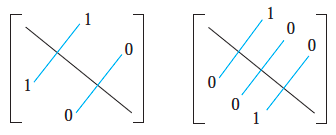
\includegraphics[scale=0.75]{aulas/imagens/62}
	\caption{A matriz zero-um para uma relação simétrica e antissimétrica.}
	\label{Figura62}
\end{figure}

Suppose that the relation R on a set is represented by the matrix

\begin{description}
	\item[Exemplo 3]{Suponha que a relação $R$ é representada pela matriz}
\end{description}
\[
	M_R = \begin{bmatrix}
	1 & 1 & 0\\
	1 & 1 & 1\\
	0 & 1 & 1
	\end{bmatrix}?
\]

$R$ é reflexiva, simétrica e/ou antisimétrica?

\emph{Solução:} Como todas os elementos das diagonais nesta matriz são iguais a $1$, $R$ é reflexiva.
Além do mais, como $M_R$ é simétrica, então $R$ é simétrica. É também fácil notar que $R$ não é antissimétrica.


As operações booleanas estudados anteriormente também podem ser utilizados para encontrar as matrizes que 
representam a união e a intersecção de duas relações. Suponha que $R_1$ e $R_2$ são relações num conjunto $A$
representada pelas matrizes $M_{R_1}$ e $M_{R_2}$, respectivamente. A matriz que representa a união destas duas
relações possui o valor $1$ nas posições em que  $M_{R_1}$ ou $M_{R_2}$ possuem o valor $1$. A matriz que representa a
intersecção destas duas relações possui o valor $1$ nas posições em que  $M_{R_1}$ e $M_{R_2}$ possuem o valor $1$.
Sendo assim, as matrizes que representam a união e a intersecção destas duas relações são

$M_{R_1 \cup R_2} = M_{R_1} \lor M_{R_2}$ e $M_{R_1 \cap R_2} = M_{R_1} \land M_{R_2}$

\subsection{Representação de relações por meio de grafos direccionados}

Vimos anteriormente que uma relação pode ser representada por uma listagem de todos os seus pares ordenados ou por meio
de uma matriz zero-um. Existe outra forma importante de representar uma relação utilizando uma representação 
pictural. Cada elemente do conjunto é representado por um ponto, e cada par ordenado é representado utilizando um arco
cuja direcção indicada por uma seta. Utilizamos essa representação sempre que utilizamos uma relação num conjunto finito como
um grafo direccionado ou dígrafos.


\begin{description}
	\item[Definição 1]{Um \emph{grafo direccionado}, ou \emph{dígrafo}, consiste num conjunto $V$ de \emph{vértices} 
	(ou \emph{nós}) e um conjunto $E$ pares ordenados dos elementos de $V$ chamados de \emph{arestas} (ou \emph{arcos}). 
	O vértice $a$ é chamado de \emph{vértice inicial} da aresta $(a,b)$, e o vértice $b$ é chamado de \emph{vértice terminal}
	desta aresta.}
\end{description}

Uma aresta da forma $(a, a)$ é representada utilizando um arco do vértice $a$ de volta à sí mesmo. Tal aresta é chamada de 
\textbf{laço} ou \textbf{loop}.


\begin{description}
	\item[Exemplo 4]{O grafo direccionado com os vértices $a, b, c$ e $d$ e as arestas $(a,b), (a,d), (b,b), (b,d), (c,a)
	(c,b)$ e $(d,b) é apresentado na Figura \ref{Figura63}$
	}
\end{description}

\begin{figure}[H]
	\centering
	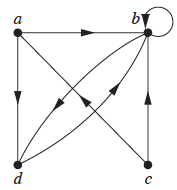
\includegraphics[scale=0.75]{aulas/imagens/63}
	\caption{Um grafo direccionado.}
	\label{Figura63}
\end{figure}


A relação $R$ no conjunto $A$ é representada pelo grafo ordenado que possui elementos de $A$ como seus vértices e os pares 
ordenados $(a,b)$, onde $(a,b) \in R$, como arestas. Esta atribuição configura uma correspondência um-para-um entre as relações
no conjunto $A$ e os grafos direcionados que possuem $A$ como o seu conjunto de vértices. Assim, cada afirmação sobre relações
corresponde a uma afirmação sobre grafos direccionados, e vice-versa. Grafos direccioandos fornecem uma exibição visual das
relações e por isso são utilizados no estudo das relações e de suas propriedades. A utilização de grafos direccionados 
na represetntação de relações num conjunto é ilustrada nos seguintes exemplos.

The directed graph of the relation

on the set {1, 2, 3, 4} is shown in Figure 4.


\begin{description}
	\item[Exemplo 5]{
	O grafo direccionado da relação\\
	$R = {(1, 1), (1, 3), (2, 1), (2, 3), (2, 4), (3, 1), (3, 2), (4, 1)}$\\
	no conjunto ${1, 2, 3, 4}$ é ilustrado na Figura \ref{Figura64}
	}
\end{description}

\begin{figure}[H]
	\centering
	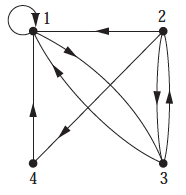
\includegraphics[scale=0.75]{aulas/imagens/64}
	\caption{Um grafo direccionado.}
	\label{Figura64}
\end{figure}

\begin{description}
	\item[Exemplo 6]{
	Quais são os pares ordenados na relação $R$ que representada pelo grafo direccionado da Figura \ref{Figura65}}
\end{description}

\begin{figure}[H]
	\centering
	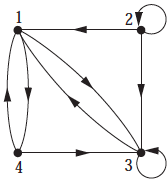
\includegraphics[scale=0.75]{aulas/imagens/65}
	\caption{Um grafo direccionado da relação R.}
	\label{Figura65}
\end{figure}

\emph{Solução:} Os pares ordenados $(x,y)$ na relação na relação são\\
$R = {(1, 3), (1, 4), (2, 1), (2, 2), (2, 3), (3, 1), (3, 3), (4, 1), (4, 3)}$

Cada um destes pares corresponde à uma aresta do grafo direccionado sendo $(2,2)$ e $(3,3)$ dois laços.

O grafo direccionado que representa uma relação pode ser utilizado para determinar se a relação possui certas propriedades.
Por exemplo, a relação é reflexiva se e somente se existe um laço em cada vértice do grafo direccionado, de tal forma que
todos os pares ordenados da forma $(x,x)$ ocorrem na relação. A relação é simétrica se e somente se para cada aresta entre vértices
distintos no digrafo existe uma aresta na direcção oposta, tal que $(y,x)$ existe na relação sempre que $(x,y)$ existe na
relação. Da mesma forma, uma relação é antissimétrica se e somente se não existem duas arestas
em direcções opostas entre vértices distintos. Finalmente, uma relação é transitiva se e somente se sempreque
que existe uma aresta de um vértice $x$ para um vértice $y$ e uma aresta de um vértice $y$ para um vértice $z$, existe uma
aresta de $x$ para $z$ (completando um triângulo onde cada lado é aresta direccionada correctamente).


\begin{description}
	\item[Exemplo 7]{Determine se os grafos direccionados apresentados nas Figuras \ref{Figura66} e \ref{Figura67} são
	reflexivos, simétricos, antissimétricos e/ou transitivos}.
\end{description}

\begin{figure}[H]
	\centering
	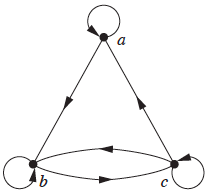
\includegraphics[scale=0.75]{aulas/imagens/66}
	\caption{Um grafo direccionado da relação R.}
	\label{Figura66}
\end{figure}

\begin{figure}[H]
	\centering
	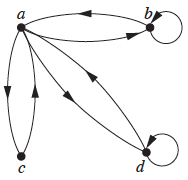
\includegraphics[scale=0.75]{aulas/imagens/67}
	\caption{Um grafo direccionado da relação S.}
	\label{Figura67}
\end{figure}

\emph{Solução:} Como existem laços em todos os vértices do grafo direccionado de $R$, ele é reflexivo. $R$ não é simétrica
nem anti-simétrica porque existe uma aresta de $a$ para $b$ mas não de $b$ para $a$, mas existem arestas em ambas direcções
que conectam $b$ e $c$. Finalmente, $R$ não é transitiva porque existe uma aresta de $a$ para $b$ e uma aresta de $b$ para $c$,
mas não existe uma aresta de $a$ para $c$. Como não existem laços em todo os vértices do grafo direccionado de S, esta relação não é reflexiva. É simétrica
mas não antissimétrica, porque cada aresta entre vértices distintos é acompanhada por uma aresta na direcção oposta. Não é
díficil notar também que o grafo direccionado de $S$ não é transitivo, porque $(c,a)$ e $(a,b)$ pertencem a $S$, mas
$(c,b)$ não pertence a $S$.

Estudaremos os grafos em mais detalhnes no próximo capítulo.


\section{Fechamento de relações}

\subsection{Introdução}

Uma rede de computadores de uma empresa possui centros de dados em Benguela, Bengo, Cabinda, Cunene, Huíla e Luanda.
Existem ligações directas de Benguela para o Bengo, de Benguela para o Bengo, de Benguela para Cunene, do Bengo para o
Cunene, de Cunene para Cabinda e da Huíla para Luanda. Seja $R$ a relação que contém $(a,b)$ se existe uma ligação do 
centro de dados em $a$ com o centro de dados em $b$, como podemos determinar se existe uma ligação (possívelmente indirecta)
composta de uma ou mais linhas de um centro para outro? Como nem todas as ligações são directas, tal como a ligação de
Benguela para Cabinda que passa por Cunene, $R$ não pode ser utilizada directamente para responder esta questão.
Na linguagem das relações, $R$ não é transitiva, portanto não contém todos os pares que podem ser ligado. Tal como iremos
mostrar nesta secção, é possível achar todos os pares de centros de dados que possuem um link por construír
uma relação transitiva $S$ que contém $R$ tal que $S$ é um subconjunto de todas as relações transitivas que contêm $R$.


\section{Relações de equivalência}

\section{Ordens parciais}

\subsection{Exercícios}
\chapter*{Relações}
%%1

\section*{Relações e suas propriedades}

For each of these relations on the set {1, 2, 3, 4}, decide
whether it is reflexive, whether it is symmetric, whether
it is antisymmetric, and whether it is transitive.

\begin{enumerate}
  	\item {Liste os pares ordendados na relação $R$ de $A = \{0,1,2,3,4\}$ para $B = \{0,1,2,3\}$ onde $(a,b) \in R$ se
  	e somente se}
  	\begin{enumerate}
  	  	\item $a = b$ \item $a + b = 4$ \item $a > b$ \item $a | b$ \item $mdc(a,b)=1$ \item $mmc(a,b)=2$
  	\end{enumerate}
  	
  	\item{Para cada uma das relações no conjunto $\{1,2,3,4\}$ indiqye se são: reflexivas, simétricas, antissimétricas
  	e transitivas}
  	\begin{enumerate}
  	  	\item $\{(2, 2), (2, 3), (2, 4), (3, 2), (3, 3), (3, 4)\}$
  	  	\item $\{(1, 1), (1, 2), (2, 1), (2, 2), (3, 3), (4, 4)\}$
  	  	\item $\{(2, 4), (4, 2)\}$
  	  	\item $\{(1, 2), (2, 3), (3, 4)\}$
  	  	\item $\{(1, 1), (2, 2), (3, 3), (4, 4)\}$
  	  	\item $\{(1, 3), (1, 4), (2, 3), (2, 4), (3, 1), (3, 4)\}$
  	\end{enumerate}
 a is taller than b.
b) a and b were born on the same day.
c) a has the same first name as b.
d) a and b have a common grandparent.

  	\item {Determine se a relação $R$ conjunto de todas as pessoas é reflexiva, simétrica, antissimétrica, e/ou
  	transitiva, onde $(a,b) \in R$ se e somente se}
  	\begin{enumerate}
  		\item $a$ é mais alto que $b$ \item $a$ e $b$ onde 
  	\end{enumerate}	
\end{enumerate}

\section*{Representação de relações}

\begin{enumerate}
  	
\end{enumerate}

\vspace*{2em}
\begin{center}\textbf{Continua!!! (Mais exercícios)}\end{center}
\chapter{Grafos}
\chapter*{Exercícios - Conjuntos e funções}
%%1

\section*{Conjuntos}

\begin{enumerate}
  	\item Seja $A$ o conjunto dos estudantes que vivem à $5 km$ do campus e $B$ o conjunto dos estudantes que vêm 
  	de bicicleta às aulas. Descreva os estudantes em cada um dos seguintes conjuntos.
  	\begin{enumerate}
  	  	\item $A \cap B$ \item $A \cup B$ \item $A - B$ \item $B - A$
  	\end{enumerate}
  	
  	\item Liste os elementos dos seguintes conjuntos:
  	\begin{enumerate}
  		 \item $\{x | x \in \mathbb{N} \land x^2 < 25\}$ \item $\{x | x$ é um dos antigos vencedores da Fórmula 1 $\}$
  		 \item $\{x | x \in \mathbb{R} \land x^2 = -1\}$ \item $\{x | x \in \mathbb{N} \land x^2 - 5x + 6 = 0\}$
	\end{enumerate}
	
	\item Qual é cardinalidade de cada um dos seguintes conjuntos?
	\begin{enumerate}
	  	\item $ S = \{a, \{a, \{a\}\}\}$ \item $\{\{a\}, \{\{a\}\}\}$ \item $\{a, \{\emptyset \}, \emptyset\}$
	  	\item $\{\emptyset, \{\emptyset, \{\emptyset\}\},\{\emptyset, \{\emptyset, \{\emptyset\}\}\}\}$
	\end{enumerate}
	
  	\item Suponha que $A$ é o conjunto dos estudantes do segundo ano e $B$ é o conjunto dos estudantes de Lógica de Programação.
  	Descreva cada um dos conjuntos em termos de $A$ e $B$.
  	\begin{enumerate}
  		\item O conjunto dos estudantes do segundo ano com a cadeira de Lógica de Programação
  		\item O conjunto dos estudantes do segundo ano que não têm a cadeira de Lógica de Programação
  		\item O conjunto dos estudantes que são, ou do segundo ano ou têm a cadeira de Lógica de Programação
  		\item O conjunto dos estudantes que não são do segundo ano, nem têm a cadeira de Lógica de Programação
	\end{enumerate}

	\item Sejam, $A = \{a, b, c, d, e\}$ e $B = \{a, b, c, d, e, f, g, h\}$ encontre:
	\begin{enumerate}
	  \item $A \cup B$ \item $A \cap B$ \item $A - B$ \item $B - A$ 
	\end{enumerate}
	
	\item Desenhe os diagramas de Venn para cada uma das seguintes combinações dos domínios A, B e C
	\begin{enumerate}
		\item $A \cap (B \cup C)$ \item $A \cap B \cap C$ \item $(A - B) \cup (A - C) \cup (B - C)$ 
		\item $A \cap (B - C)$ \item $(A \cap B) \cup (A \cap C)$ \item $(A \cap B) \cup (A \cap C)$
	\end{enumerate}
\end{enumerate}

\section*{Funções}

\begin{enumerate}
	\item Determine se $f$ é uma função de $\mathbb{Z}$ em $\mathbb{R}$ se
	\begin{enumerate}
		\item $f(n) = \pm n$ \item $\sqrt{n^2 + 1}$ \item $\frac{1}{(n^2 - 4)}$  
	\end{enumerate}
	
	\item Determine se as seguintes funções de $\mathbb{Z}$ para $\mathbb{Z}$ são injectivas ou sobrejectivas.
	\begin{enumerate}
	  	\item $f(n) = n - 1$ \item $f(n) = n^2 + 1$ \item $f(n) = n^3$ \item $f(n) = \frac{n}{2}$
	\end{enumerate}
	
	\item Considere as seguintes funções do conjunto dos estudantes de Estruturas Discretas. Em que condições uma função é injectiva
	se ela atribui a um estudante o seu:
	\begin{enumerate}
	  	\item Número de telemóvel
	   	\item Número de estudante
	   	\item Nota final
	   	\item Local de Nascimento
	\end{enumerate}

	\begin{description}
		\item[Definição 1] Uma função diz-se \emph{bijectiva} quando é ao mesmo tempo injectiva (um para um) e sobrejectiva.
		\item[Exemplo 1] Seja $f$ uma função da forma $\{a,b,c,d\}$ para $\{1,2,3,4\}$ com $f(a) = 4, f(b) = 2, f(c) = 1$ e $f(d) = 3$.
		A função $f$ é uma função injectiva e sobrejectiva. É injectiva porque não existem valores no domínio que são mapeados
		para o mesmo valor no co-domínio. É sobrejectiva porque todos os quatro elementos do co-domínio são imagens dos elementos
		no domínio. Então $f$ é uma função \emph{bijectiva} ou uma \emph{bijeção}.	
	\end{description}
	
	\item Determina se cada uma das seguintes funções é uma bijeção de $\mathbb{R}$ para $\mathbb{R}$.
	\begin{enumerate}
		\item $f(x) = -3x + 4$ \item $f(x) = -3x^2 + 7$ \item $f(x) = (x+1)/(x+2)$ \item $f(x) = x^5 + 1$ \item $f(x) = 2x + 1$
		\item $f(x) = x^2 + 1$
	\end{enumerate}
	
	\begin{description}
		\item[Definição 2] Seja $f$ a função de $A$ para $B$ e seja $S$ um subconjunto de $A$. A imagem de $S$ sobre a função $f$ é o
		subconjunto de $B$ que consiste nas imagens dos elementos de $S$. Denotamos a imagem de $S$ por $f(S)$, tal que
		$f(S) = \{t | \exists s \in S(t = f(s))\}$. Também podemos utilizar a representação $\{f(s) | s \in S\}$
		\item[Exemplo 2] Seja $A = \{a,b,c,d,e\}$ e $B = \{1,2,3,4\}$ com $f(a)=2, f(b)=1, f(c)=4, f(d)=1$, e $f(e)=1$. A imagem
		do subconjunto $S = \{b,c,d\}$ é o conjunto $f(S) = \{1, 4\}$.
	\end{description}

	\item Seja $S = \{-1,0,2,4,7\}$ encontre $f(S)$ se
	\begin{enumerate}
	  	\item $f(x)=1$ \item $f(x)=2x + 1$ \item $f(x)=\lceil \frac{x}{5} \rceil$ \item $f(x) = \lfloor \frac{(x^2 + 1)}{3} \rfloor$  
	\end{enumerate}

	\item Seja $f(x) = \lfloor \frac{x^2}{3} \rfloor$, encontre $f(S)$ se,
	\begin{enumerate}
		\item $S = \{-2,-1,0,1,2,3\}$ \item $S=\{0,1,2,3,4,5\}$ \item $S=\{1,5,7,11\}$ \item $S=\{2,6,10,14\}$ 
	\end{enumerate}
	
	\item Seja $f: \mathbb{N} \to \mathbb{N}$ definida por $f(x) = x + 1$. Seja $g: \mathbb{N} \to \mathbb{N}$ definida por $g(x) = 3x$.
	Calcule o seguinte:
	\begin{enumerate}
	  	\item $(g \circ f)(5)$ \item $(f \circ g)(5)$ \item $(g \circ f)(x)$ \item $(f \circ g)(x)$ \item $(f \circ f)(x)$
	  	\item $(g \circ g)(x)$
	\end{enumerate}
	
	\item Para cada uma das seguintes bijeções $f: \mathbb{R} \to \mathbb{R}$, encontre $f^{-1}$
	\begin{enumerate}
	  	\item $f(x)=7x$ \item $f(x) = x^3$ \item $f(x) = \frac{(x + 4)}{3}$
	\end{enumerate}
\end{enumerate}

\vspace*{2em}
\begin{center}\textbf{Continua!!! (Mais exercícios)}\end{center}
\chapter{Árvores}
\chapter*{Exercícios - Conjuntos e funções}
%%1

\section*{Conjuntos}

\begin{enumerate}
  	\item Seja $A$ o conjunto dos estudantes que vivem à $5 km$ do campus e $B$ o conjunto dos estudantes que vêm 
  	de bicicleta às aulas. Descreva os estudantes em cada um dos seguintes conjuntos.
  	\begin{enumerate}
  	  	\item $A \cap B$ \item $A \cup B$ \item $A - B$ \item $B - A$
  	\end{enumerate}
  	
  	\item Liste os elementos dos seguintes conjuntos:
  	\begin{enumerate}
  		 \item $\{x | x \in \mathbb{N} \land x^2 < 25\}$ \item $\{x | x$ é um dos antigos vencedores da Fórmula 1 $\}$
  		 \item $\{x | x \in \mathbb{R} \land x^2 = -1\}$ \item $\{x | x \in \mathbb{N} \land x^2 - 5x + 6 = 0\}$
	\end{enumerate}
	
	\item Qual é cardinalidade de cada um dos seguintes conjuntos?
	\begin{enumerate}
	  	\item $ S = \{a, \{a, \{a\}\}\}$ \item $\{\{a\}, \{\{a\}\}\}$ \item $\{a, \{\emptyset \}, \emptyset\}$
	  	\item $\{\emptyset, \{\emptyset, \{\emptyset\}\},\{\emptyset, \{\emptyset, \{\emptyset\}\}\}\}$
	\end{enumerate}
	
  	\item Suponha que $A$ é o conjunto dos estudantes do segundo ano e $B$ é o conjunto dos estudantes de Lógica de Programação.
  	Descreva cada um dos conjuntos em termos de $A$ e $B$.
  	\begin{enumerate}
  		\item O conjunto dos estudantes do segundo ano com a cadeira de Lógica de Programação
  		\item O conjunto dos estudantes do segundo ano que não têm a cadeira de Lógica de Programação
  		\item O conjunto dos estudantes que são, ou do segundo ano ou têm a cadeira de Lógica de Programação
  		\item O conjunto dos estudantes que não são do segundo ano, nem têm a cadeira de Lógica de Programação
	\end{enumerate}

	\item Sejam, $A = \{a, b, c, d, e\}$ e $B = \{a, b, c, d, e, f, g, h\}$ encontre:
	\begin{enumerate}
	  \item $A \cup B$ \item $A \cap B$ \item $A - B$ \item $B - A$ 
	\end{enumerate}
	
	\item Desenhe os diagramas de Venn para cada uma das seguintes combinações dos domínios A, B e C
	\begin{enumerate}
		\item $A \cap (B \cup C)$ \item $A \cap B \cap C$ \item $(A - B) \cup (A - C) \cup (B - C)$ 
		\item $A \cap (B - C)$ \item $(A \cap B) \cup (A \cap C)$ \item $(A \cap B) \cup (A \cap C)$
	\end{enumerate}
\end{enumerate}

\section*{Funções}

\begin{enumerate}
	\item Determine se $f$ é uma função de $\mathbb{Z}$ em $\mathbb{R}$ se
	\begin{enumerate}
		\item $f(n) = \pm n$ \item $\sqrt{n^2 + 1}$ \item $\frac{1}{(n^2 - 4)}$  
	\end{enumerate}
	
	\item Determine se as seguintes funções de $\mathbb{Z}$ para $\mathbb{Z}$ são injectivas ou sobrejectivas.
	\begin{enumerate}
	  	\item $f(n) = n - 1$ \item $f(n) = n^2 + 1$ \item $f(n) = n^3$ \item $f(n) = \frac{n}{2}$
	\end{enumerate}
	
	\item Considere as seguintes funções do conjunto dos estudantes de Estruturas Discretas. Em que condições uma função é injectiva
	se ela atribui a um estudante o seu:
	\begin{enumerate}
	  	\item Número de telemóvel
	   	\item Número de estudante
	   	\item Nota final
	   	\item Local de Nascimento
	\end{enumerate}

	\begin{description}
		\item[Definição 1] Uma função diz-se \emph{bijectiva} quando é ao mesmo tempo injectiva (um para um) e sobrejectiva.
		\item[Exemplo 1] Seja $f$ uma função da forma $\{a,b,c,d\}$ para $\{1,2,3,4\}$ com $f(a) = 4, f(b) = 2, f(c) = 1$ e $f(d) = 3$.
		A função $f$ é uma função injectiva e sobrejectiva. É injectiva porque não existem valores no domínio que são mapeados
		para o mesmo valor no co-domínio. É sobrejectiva porque todos os quatro elementos do co-domínio são imagens dos elementos
		no domínio. Então $f$ é uma função \emph{bijectiva} ou uma \emph{bijeção}.	
	\end{description}
	
	\item Determina se cada uma das seguintes funções é uma bijeção de $\mathbb{R}$ para $\mathbb{R}$.
	\begin{enumerate}
		\item $f(x) = -3x + 4$ \item $f(x) = -3x^2 + 7$ \item $f(x) = (x+1)/(x+2)$ \item $f(x) = x^5 + 1$ \item $f(x) = 2x + 1$
		\item $f(x) = x^2 + 1$
	\end{enumerate}
	
	\begin{description}
		\item[Definição 2] Seja $f$ a função de $A$ para $B$ e seja $S$ um subconjunto de $A$. A imagem de $S$ sobre a função $f$ é o
		subconjunto de $B$ que consiste nas imagens dos elementos de $S$. Denotamos a imagem de $S$ por $f(S)$, tal que
		$f(S) = \{t | \exists s \in S(t = f(s))\}$. Também podemos utilizar a representação $\{f(s) | s \in S\}$
		\item[Exemplo 2] Seja $A = \{a,b,c,d,e\}$ e $B = \{1,2,3,4\}$ com $f(a)=2, f(b)=1, f(c)=4, f(d)=1$, e $f(e)=1$. A imagem
		do subconjunto $S = \{b,c,d\}$ é o conjunto $f(S) = \{1, 4\}$.
	\end{description}

	\item Seja $S = \{-1,0,2,4,7\}$ encontre $f(S)$ se
	\begin{enumerate}
	  	\item $f(x)=1$ \item $f(x)=2x + 1$ \item $f(x)=\lceil \frac{x}{5} \rceil$ \item $f(x) = \lfloor \frac{(x^2 + 1)}{3} \rfloor$  
	\end{enumerate}

	\item Seja $f(x) = \lfloor \frac{x^2}{3} \rfloor$, encontre $f(S)$ se,
	\begin{enumerate}
		\item $S = \{-2,-1,0,1,2,3\}$ \item $S=\{0,1,2,3,4,5\}$ \item $S=\{1,5,7,11\}$ \item $S=\{2,6,10,14\}$ 
	\end{enumerate}
	
	\item Seja $f: \mathbb{N} \to \mathbb{N}$ definida por $f(x) = x + 1$. Seja $g: \mathbb{N} \to \mathbb{N}$ definida por $g(x) = 3x$.
	Calcule o seguinte:
	\begin{enumerate}
	  	\item $(g \circ f)(5)$ \item $(f \circ g)(5)$ \item $(g \circ f)(x)$ \item $(f \circ g)(x)$ \item $(f \circ f)(x)$
	  	\item $(g \circ g)(x)$
	\end{enumerate}
	
	\item Para cada uma das seguintes bijeções $f: \mathbb{R} \to \mathbb{R}$, encontre $f^{-1}$
	\begin{enumerate}
	  	\item $f(x)=7x$ \item $f(x) = x^3$ \item $f(x) = \frac{(x + 4)}{3}$
	\end{enumerate}
\end{enumerate}

\vspace*{2em}
\begin{center}\textbf{Continua!!! (Mais exercícios)}\end{center}
\chapter*{Consideraçõres finais}

\end{document}